\subsection{UC1 - Inserimento dei dati }
\label{uc1}

    \begin{figure}[htbp]
        \centering
        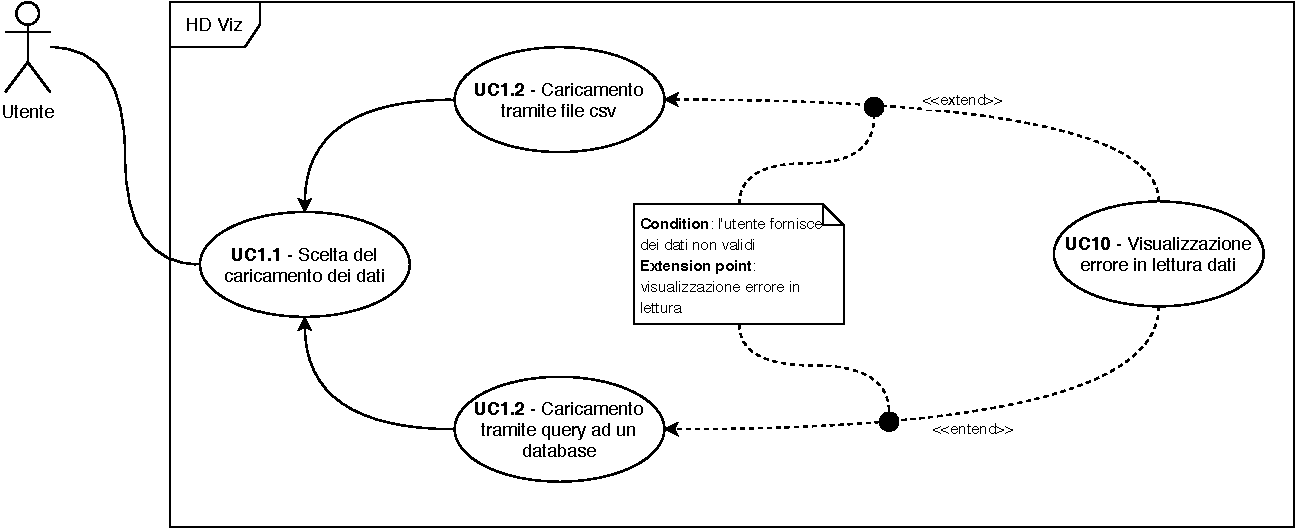
\includegraphics[width=1.0\textwidth]{source/sections/casi-uso/diagrams/uc1.pdf}
        \caption{UC1 - Inserimento dei dati}
        % \label{fig:uc1}
    \end{figure}
    
    \begin{itemize}
    \item \textbf{Attore}: Utente
    \item \textbf{Descrizione}: L'utente carica i dati per ottenere una visualizzazione
    \item \textbf{Precondizione}:
    \begin{itemize}
        \item Il sistema è funzionante e raggiungibile
        \item L'utente accede alla pagina dell'applicazione
    \end{itemize}
    \item \textbf{Postcondizione}: I dati sono stati caricati correttamente come matrice $N\times M$
    \item \textbf{Scenario Principale}: 
        \begin{enumerate}
            \item L'utente accede alla pagina dell'applicazione
            \item L'utente sceglie come caricare i dati (\hyperref[uc1.1]{UC1.1}):
                \begin{enumerate}
                    \item l'utente ha scelto di ricavare i dati caricando un file csv
                    \item l'utente ha scelto di ricavare i dati tramite una query a un database
                \end{enumerate}
        \end{enumerate}  
    \item \textbf{Estensioni}:
        \begin{enumerate}
            \item L'utente inserisce dei dati non validi o non nel formato corretto:
                \begin{enumerate}
                    \item fallisce l'inserimento dei dati
                    \item viene visualizzato un messaggio di errore in lettura dei dati (\hyperref[uc10]{UC10}):
                \end{enumerate}
        \end{enumerate}  
    \item \textbf{Generalizzazioni}:
        \begin{enumerate}
            \item L'utente sceglie come caricare i dati
                \begin{enumerate}
                    \item caricando un file csv (\hyperref[uc1.2]{UC1.2})
                    \item tramite una query a un database (\hyperref[uc1.3]{UC1.3})
                \end{enumerate}
        \end{enumerate}  
    \end{itemize}
    
    %%%
    \subsubsection{UC1.1 - Scelta del caricamento dei dati}
    \label{uc1.1}
    
    \begin{itemize}
    \item \textbf{Attore}: Utente
    \item \textbf{Descrizione}: L'utente sceglie come caricare i dati
    \item \textbf{Precondizione}:
    \begin{itemize}
        \item Il sistema è funzionante e raggiungibile
        \item L'utente accede alla pagina dell'applicazione
    \end{itemize}
    \item \textbf{Postcondizione}: L'utente ha fatto la scelta
    \item \textbf{Scenario Principale}: 
        \begin{enumerate}
            \item L'utente sceglie come caricare i dati in base alle proprie esigenze
        \end{enumerate}
    \end{itemize}
    
    %%%
    \subsubsection{UC1.2 - Caricamento tramite file csv}
    \label{uc1.2}
    
    \begin{itemize}
    \item \textbf{Attore}: Utente
    \item \textbf{Descrizione}: L'utente sceglie di caricare i dati tramite un file csv
    \item \textbf{Precondizione}:
    \begin{itemize}
        \item Il sistema è funzionante e raggiungibile
        \item L'utente accede alla pagina dell'applicazione
        \item L'utente è in possesso di un file csv contenete i dati
    \end{itemize}
    \item \textbf{Input}: File csv conenente i dati da visualizzare
    \item \textbf{Postcondizione}: L'utente ha caricato il suo file csv come matrice $N\times M$
    \item \textbf{Scenario Principale}: 
        \begin{enumerate}
            \item L'utente ha scelto di inserire i file tramite un file csv
            \item Tramite l'apposito bottone sceglie il file
        \end{enumerate}
        \item \textbf{Estensioni}:
        \begin{enumerate}
            \item L'utente inserisce dei dati non validi o non nel formato corretto:
                \begin{enumerate}
                    \item fallisce l'inserimento dei dati
                    \item viene visualizzato un messaggio di errore in lettura dei dati (\hyperref[uc10]{UC10}):
                \end{enumerate}
        \end{enumerate}  
    \end{itemize}

    
    %%%
    \subsubsection{UC1.3 - Caricamento tramite query ad un database}
    \label{uc1.3}
    
    \begin{itemize}
    \item \textbf{Attore}: Utente
    \item \textbf{Descrizione}: L'utente sceglie di caricare i dati tramite tramite query ad un database
    \item \textbf{Precondizione}:
    \begin{itemize}
        \item Il sistema è funzionante e raggiungibile
        \item L'utente accede alla pagina dell'applicazione
        \item L'utente può collegarsi ad un database (possiede le credenziali)
    \end{itemize}
    \item \textbf{Postcondizione}: L'utente si è collegato al database e ha recuperato i dati tramite query come matrice $N\times M$
    \item \textbf{Scenario Principale}: 
        \begin{enumerate}
            \item L'utente ha scelto di caricare i dati tramite tramite query ad un database in cui può collegarsi
            \item Inserisce le credenziali, e scrive la sua query per ricavare i dati
        \end{enumerate}
        \item \textbf{Estensioni}:
        \begin{enumerate}
            \item L'utente inserisce dei dati non validi o non nel formato corretto:
                \begin{enumerate}
                    \item fallisce l'inserimento dei dati
                    \item viene visualizzato un messaggio di errore in lettura dei dati (\hyperref[uc10]{UC10}):
                \end{enumerate}
        \end{enumerate}  
    \end{itemize}

    